\documentclass[a4paper,oneside]{article}
\usepackage[english]{babel}
\usepackage[utf8]{inputenc}
\usepackage{graphicx}
\usepackage{amsfonts}
\usepackage[affil-it]{authblk}
\usepackage[table]{xcolor}
\usepackage{pagecolor}
\usepackage{afterpage}
\usepackage{changepage}
\usepackage[mark]{gitinfo2}

\usepackage[a4paper, includeheadfoot]{geometry}
\geometry{a4paper, total={210mm,297mm}, left=38mm, right=38mm, top=24mm, bottom=48mm}

\usepackage{fancyhdr}
\pagestyle{fancy}

\usepackage{xcolor}
\graphicspath{ {./images/} }
\usepackage[pdftex,
    pdfauthor={Evan Green \& Adam Waldenberg, The Unigrid Foundation},
    pdftitle={Unigrid: The Next Internet Revolution},
    pdfsubject={Orange Paper},
    pdfkeywords={blockchain;internet;bitcoin;unigrid;sharding;segmentation;consensus;decentralized;governance;gridnode},
    pdfproducer={Latex with hyperref, or other system},
    pdfcreator={pdflatex, or other tool}]{hyperref}

\let\oldhref\href
\renewcommand{\href}[2]{\oldhref{#1}{\bfseries#2}}
\definecolor{txtcolor}{rgb}{0.88,0.88,0.88}
\hypersetup{colorlinks = true, urlcolor = txtcolor, citecolor = orange, linkcolor = txtcolor}

\author{\textit{Evan Green, \href{mailto:evan@unigrid.org}{evan@unigrid.org}}\\
\textit{Adam Waldenberg, \href{mailto:adam@unigrid.org}{adam@unigrid.org}}}
\affil{The Unigrid Foundation}

\title{
	\makebox[\textwidth]{\hspace{600pt}\tikz \fill[orange] (18,1.4) rectangle (0,0);}
	\vspace{60pt}
	\begin{center}
		\includesvg[height=80pt]{unigrid-wide}
	\end{center}
	\vspace{35pt}
	\textbf{The Next Internet Revolution}
	\vspace{10pt}
}
\date{\emph{Version \gitRel\hspace{5pt}(\gitCommitterDate)}}

\definecolor{headerbg}{rgb}{0,0,0.18}
\definecolor{headerbgl}{rgb}{0.07,0.07,0.24}

\usepackage[framemethod=tikz]{mdframed}
\usepackage[inkscapearea=page]{svg}

\mdfdefinestyle{unigridheader}{
	userdefinedwidth=381pt,
	backgroundcolor=headerbg,
	linecolor=orange,
	linewidth=3pt,
	leftline=false,
	rightline=false,
	bottomline=true,
	topline=false,
	innerbottommargin=0,
	innerrightmargin=0
}

\mdfdefinestyle{textimage}{
	backgroundcolor=headerbg,
	linecolor=orange,
	linewidth=3pt,
	leftline=false,
	rightline=false,
	bottomline=true,
	topline=true,
	innerrightmargin=0,
	innerleftmargin=0,
	innertopmargin=4pt,
	innerbottommargin=4pt,
	leftmargin=0
}

\setlength{\headheight}{70pt}%
\renewcommand{\headrulewidth}{0pt}
\renewcommand{\footrulewidth}{0pt}
\lhead{
	\begin{mdframed}[style=unigridheader]
		\begin{flushright}
			\includesvg[height=30pt]{unigrid-wide}
		\end{flushright}
	\end{mdframed}
}

\renewcommand{\familydefault}{\sfdefault}
\color{txtcolor}

\begin{document}

\newpagecolor{headerbg}
\clearpage\maketitle
\thispagestyle{empty}
\newpage
\vspace*{+34pt}
\begin{abstract}
\noindent The original Internet was envisioned to become an open and distributed network that was scalable and fair, allowing access to data and services without surveillance or security concerns. However, in recent years, the Internet has become increasingly centralized, controlled and monopolized by big businesses running huge data centers. This centralization has given big entities and businesses unprecedented control of the traffic and data of the network.

\begin{mdframed}[style=textimage]
	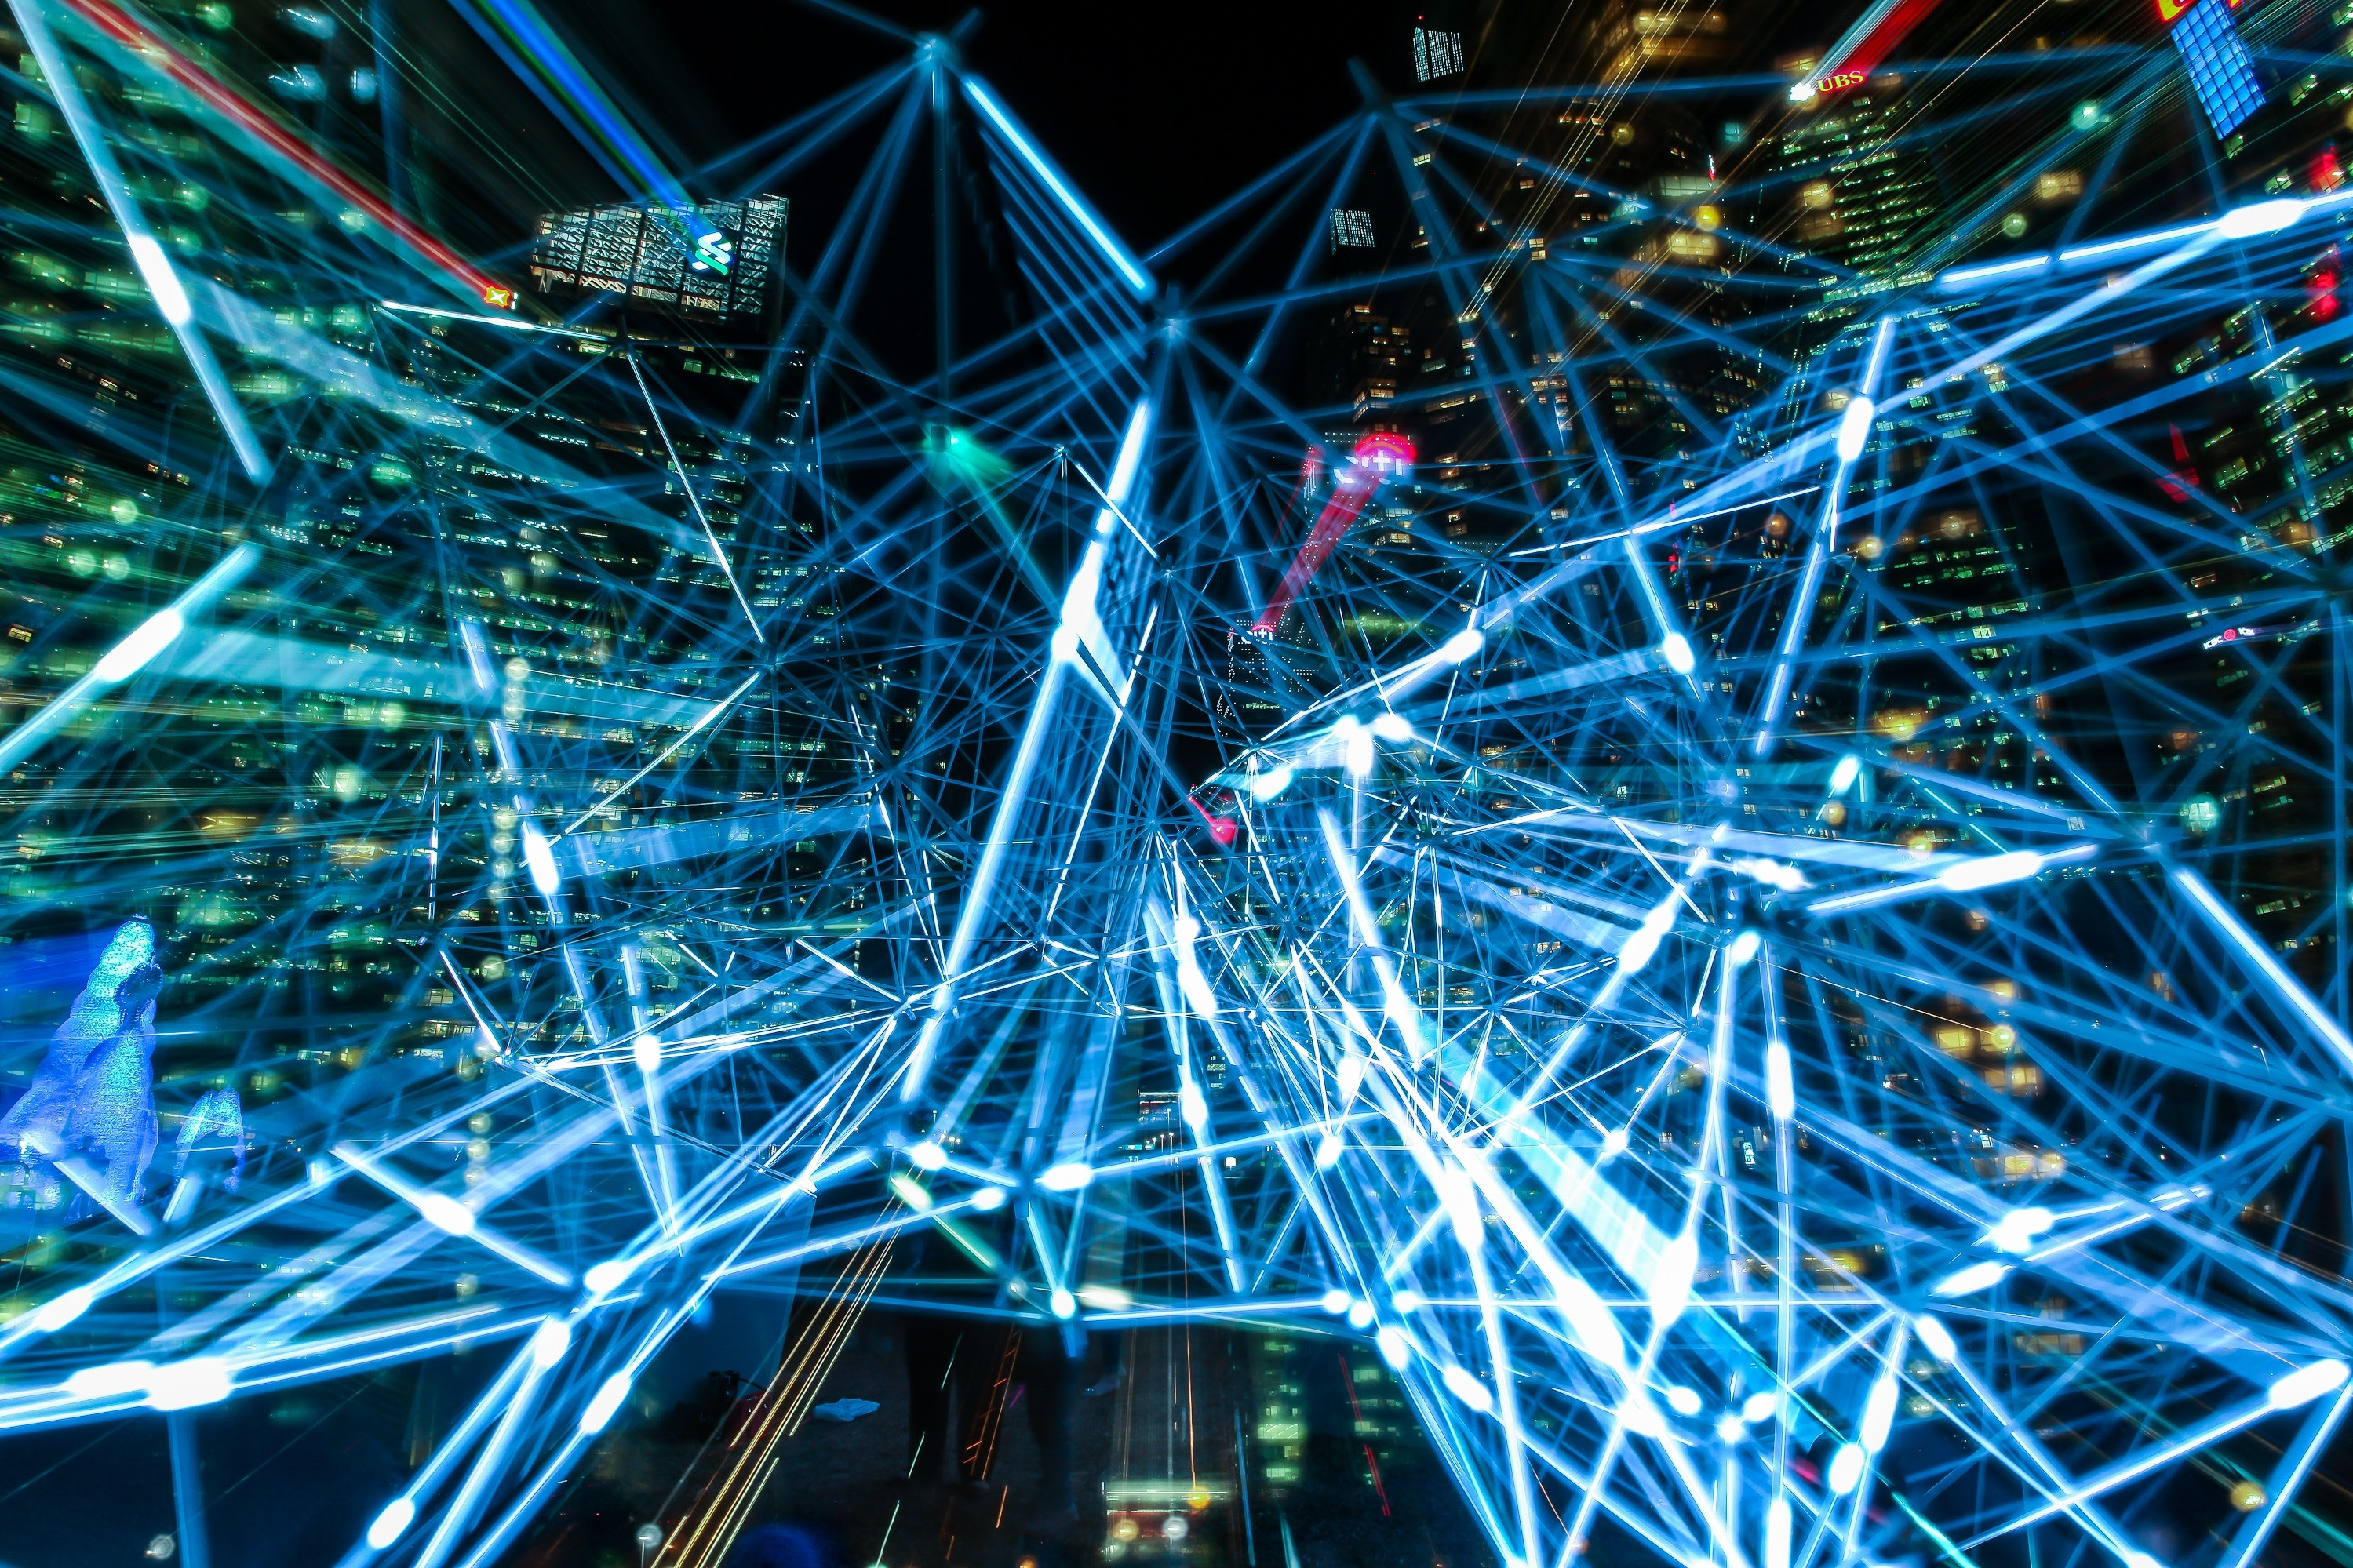
\includegraphics[width=331pt]{lights}
\end{mdframed}

\noindent With a majority of resources on the Internet owned by a minority of big corporations, these businesses are able to maintain a high cost to value ratio. The centralization and lack of fault tolerance and redundancy makes your personal data less secured. As a remedy to this deteriorating trend, we suggest the inception of a decentralized and consensus-driven segmented blockchain network based on a striped storage solution. The protocol allows for a completely decentralized and secure blockchain-based Internet where any user, including private persons, can host an income-generating service node, aiding the network with compute cycles, bandwidth, and storage space. To allow for complete utilization of the network, an access layer is provided, allowing for the development of protocols, services, and infrastructure.
\vspace*{+40pt}
\end{abstract}

\newpage
\section{Problem}
The current Internet is dominated by large multi-national conglomerates. Businesses like Google, Microsoft, and Amazon take up vast segments of the total market share. Amazon Web Services (AWS) has a dominate position, having nearly 50\% of that total market share \cite{jeb2019}.

\begin{center}

\includegraphics[width=45pt]{centralized}
\hspace{1.5cm}
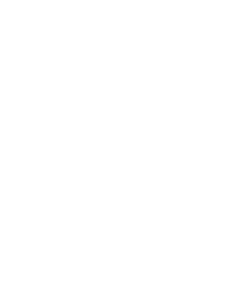
\includegraphics[width=45pt]{unreliable}
\hspace{1.5cm}
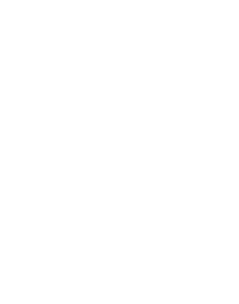
\includegraphics[width=45pt]{unsecure}
\\
\vspace{0.1cm}
\hspace{0pt}\emph{Centralized}\hspace{50pt}\emph{Unreliable}\hspace{54pt}\emph{Unsecure}\hspace{24pt}
\end{center}

\noindent A near majority of all Internet data is stored on servers owned by a single entity \cite{jeb2019}. As a consequence, this results in much of the current traffic being routed through Amazon’s servers and data centers \cite{jeb2019}. Because of this, important routes often get overloaded during peak hours, slowing down services - resulting in a degraded user experience. In fact, routes regularly become so overloaded that it effectively causes servers on the other end of the communication queue to be unreachable - something most Internet users have experienced. If your provider goes offline or gets disrupted - your service and data becomes unreachable.

\vspace{0.05cm}
\begin{mdframed}[style=textimage]
	
\includegraphics[width=381pt]{puzzle}
\end{mdframed}

\noindent The centralized nature of the resource ownership on the Internet also results in under-utilization of servers, with idle CPU cycles and gigabytes or potentially terabytes of unused storage space on a single server. This is especially true when businesses choose to cost-optimize their operations and rely on their own dedicated servers, rather than relying on the more expensive cloud provider solutions.

In some countries, Internet censorship is so prevalent that the public is limited to what news resources they are allowed to access and view \cite{wiki2021}. The original intention of the Internet was to create an open and globally accessible network, allowing everybody with access to view and take part of that information, regardless of their originating location.

For privacy, cost and security reasons, this situation is not sustainable. Hackers, oppressive governments and monopolizing businesses continuously develop better tools that infringe on your data and privacy - creating a very vulnerable situation.

\section{Discussion}
The primary goal of Unigrid is to implement an anonymous and decentralized communication solution that offers data storage and compute cycle utilization. Private individuals and businesses that value privacy or require secure data storage can take advantage of this feature.

As an example, sensitive documents such as medical records, can be stored on-chain and only shared with selected individuals or entities. The data can be shared using a key that has an expiration timer, meaning that the sharing party never has to worry about the risk that the data will be exposed or accessed by an unwanted party. It should be the owning individual or business that controls how their private data is accessed and shared. It should never be in the control of a third party - something that is usually the case today. When the data is controlled by a third party, the risk of information leaks increases dramatically. Sometimes data is stolen by hackers, other times it is leaked or shared on purpose (in secrecy or otherwise). Whatever the reason - the Unigrid network gives the control back to the user or the party that actually owns the data.

\begin{center}

\includegraphics[width=45pt]{anonymous}
\hspace{1.5cm}
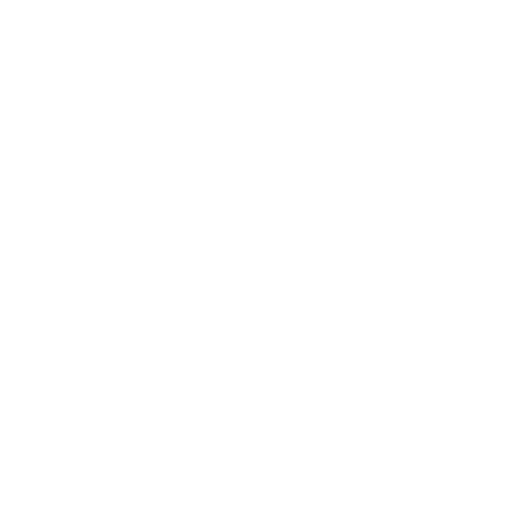
\includegraphics[width=45pt]{scalability}
\hspace{1.5cm}

\includegraphics[width=45pt]{security}
\\
\vspace{0.11cm}
\hspace{0pt}\emph{Anonymity}\hspace{49pt}\emph{Scalability}\hspace{58pt}\emph{Security}\hspace{25pt}
\end{center}

\noindent Another example is the growing IoT (Internet of Things) market. On a blockchain, the ledger is tamper-proof, removing the need for absolute trust between two communicating parties. Utilizing a blockchain network like Unigrid adds a layer of trust to the data being transmitted. On top of handling the integrity of the actual data, the network also needs to be capable of scaling without degradation when millions of IoT-connected devices join the network. As mentioned by Shruti Jain of Deloitte \cite{jain2021}, blockchain or distributed ledger technology (DLT) has the potential to help address some of the IoT security and scalability challenges.

\begin{mdframed}[style=textimage]
	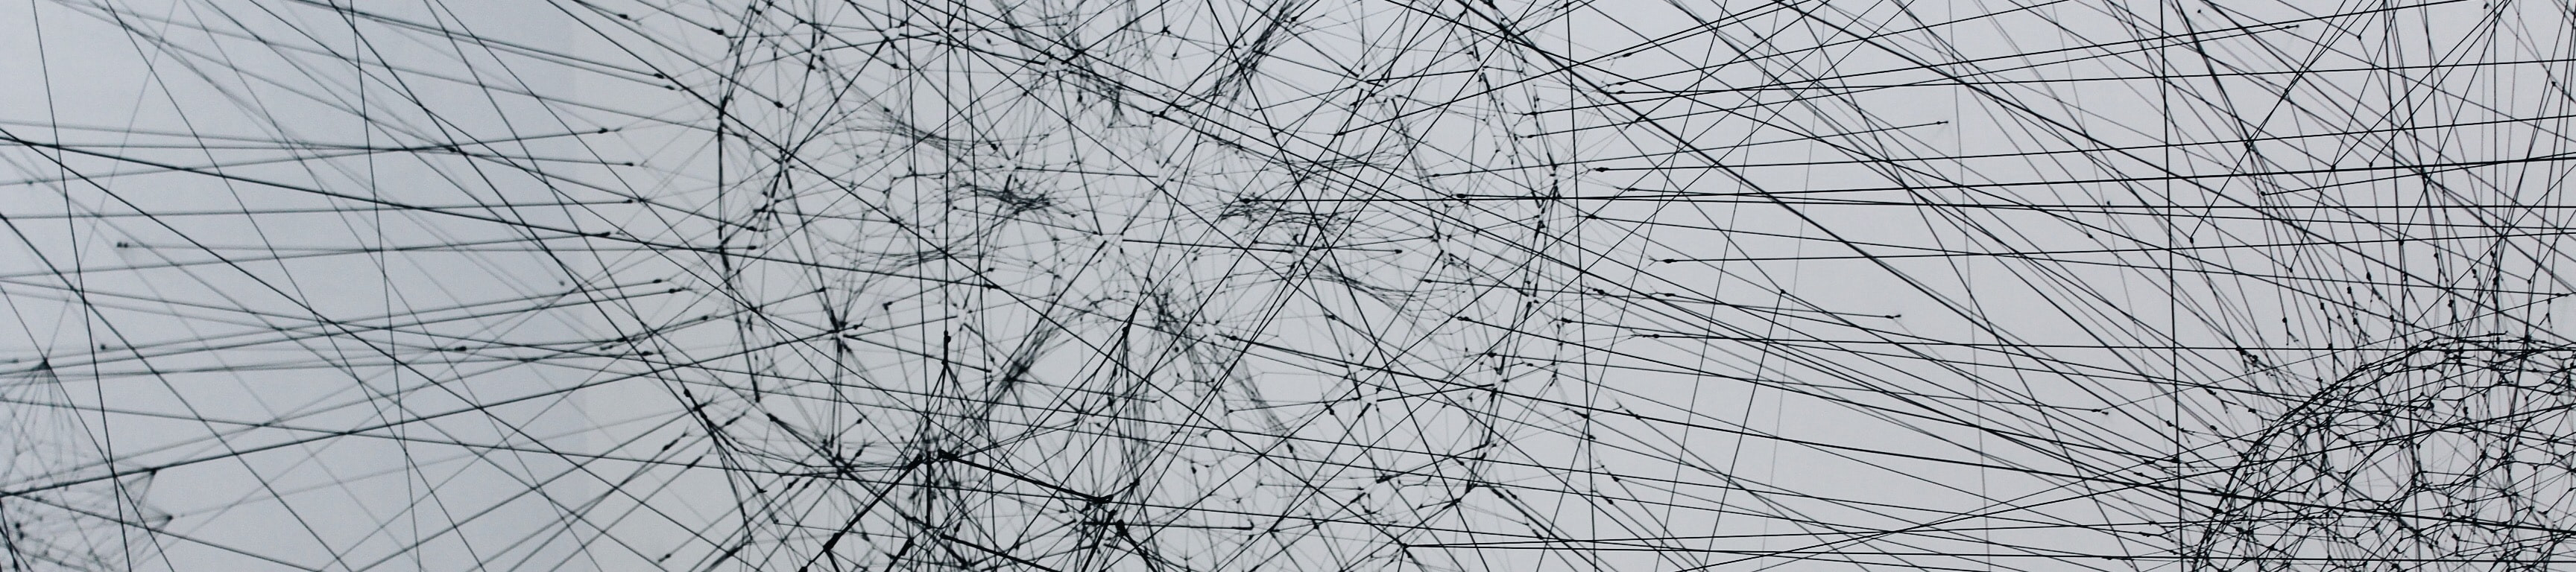
\includegraphics[width=381pt]{communication}
\end{mdframed}

\subsection{Gridnodes}
A gridnode is similar in function to a masternode as initially conceived by the Darkcoin project, where anybody can set-up a node on a server by locking up a certain amount of tokens to that node. These masternodes then provide a service to the network by contributing network bandwidth in the form of helping other nodes to synchronize and verify blocks on the network. Because these masternodes secure the network in this way, they are rewarded in tokens.

The Unigrid takes this idea further and implements gridnodes. Gridnodes are scored by the quality of the service they provide to the network and it's nodes. For example, latency, the amount of available storage capacity, processing speed and network bandwidth are all taken into account. Each gridnode is then scored based on how they rank compared to other gridnodes.

With a regular masternode, reward frequency and occurrence is based on a naively calculated list. The network simply stores this list into memory and will cycle through each block to select the next winner. With the Unigrid network and gridnodes, scoring and rewards work differently. For example, when a request is made to store data on the network, there will be a check performed - looking for the next gridnode candidate. This check will see which gridnode has received the last reward plus scan the scores of each gridnode. Once a winner is selected, this gridnode will collect the data submitted and work with the other gridnodes to shard it across the network. This sharding allows the network to scale efficiently.

\subsection{Side Chains}
The Unigrid network places blocks in appropriate side chains based on the type of work currently being sent by a communicating node. Each side chain is controlled by a group of gridnodes. A side chain is a specialized blockchain with very specific characteristics, optimized for the type of work it is meant for. For example, data storage and compute cycles don't need the brute speed that a direct communication channel requires. Therefore, the Unigrid network treats these workloads differently. The communication side chains are smaller and kept in-memory, using a very fast but less collision resistant hashing algorithm. The blockchains that handle compute cycles and storage, on the other hand, are more resistant to hash collisions - making them very secure. However, they can not handle the same throughput as the in-memory chains using the less resistant hashing variant.

\begin{center}
\vspace{0.1cm}
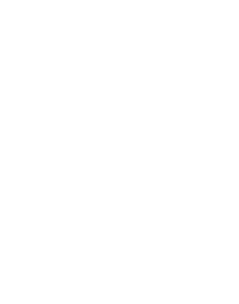
\includegraphics[width=45pt]{efficiency}
\hspace{1.5cm}

\includegraphics[width=45pt]{segmented}
\\
\vspace{0.1cm}
\hspace{10pt}\emph{Efficiency}\hspace{46pt}\emph{Segmentation}
\end{center}

\noindent The Unigrid network can create side chains on demand. The network continously rebalances, with blockchains being created, removed and restructured as the members of them and their data changes. This is possible because the network uses parity blocks and thus has the ability to rebuild side chains and throw away stale blocks.

\subsection{Data Storage}
The design of the Unigrid network allows it to store large amounts of data on-chain that can be accessed at any time. The data stored on the network is either public or private. Public data is viewable by anybody with access to the network. Private data, on the other hand, will only be accessible via a private key and has to be decrypted in order to allow access to the data.

\vspace{0.2cm}
\begin{mdframed}[style=textimage]
	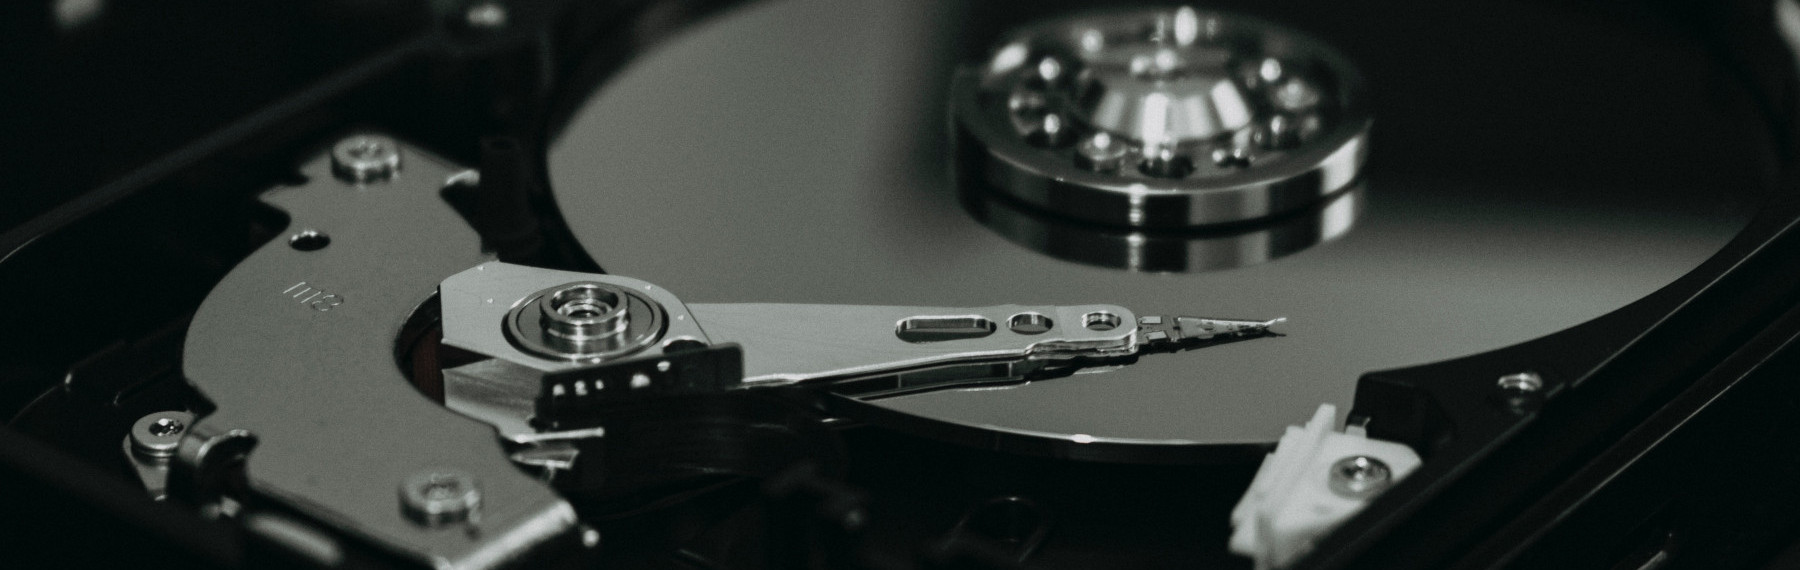
\includegraphics[width=381pt]{hard-drive}
\end{mdframed}

\noindent Cloud data storage is projected to reach a market size of \$297.54 billion by 2027 \cite{fort2021} and might even grow bigger if networks such as Unigrid reach big general adoption. Non-Fungible Tokens (NFTs) are tokens where only one specific token can be in existence at a given time. These allow for proof of ownership of a digital asset. The problem with the current system is that the only thing being stored on-chain is the actual proof of ownership. The asset itself that an NFT is tethered to is actually stored on a normal web server or some other means of storage. Consequently, if that web server or storage shuts down or is moved, the data for that NFT is lost.

The Unigrid network, is a ideal solution for handling NFTs and digital assets. Thanks to the redundancy, fault-tolerance and side chains of the network, the actual asset data can be stored in a way that ensures it can never be removed or lost by accident. This provides more long-term solution to where assets, that in some cases cost millions of dollars, are permanently and securely stored.

The NFT market has exploded in the past year. According to Joseph Young of Forbes, the market cap has grown an astounding 1758\% \cite{young2021}.

\subsection{Sharding \& Parity Blocks}
In a typical blockchain, data is stored in a vertical structure with each new block being appended to the previous block. However, this is not an ideal solution when you want to create a low latency network capable of fast data access and transfers. The solution to solve this problem on the Unigrid network involves sharding data across multiple blockchains. Furthermore, parity blocks are introduced to achieve redundancy and fault tolerance. The result is a network built for speed, security and scalability.

Sharding is a database architecture pattern related to horizontal partitioning - the practice of separating one table’s rows into multiple different tables, known as partitions \cite{mark2019}. Data on the Unigrid network will be sharded across nodes into group swarms called shard groups. This allows the network to become a self-replicating CDN (Content Delivery Network) where data is often pulled from the most optimal location. This minimizes the network latency currently experienced on the modern web where you may be pulling data from a webpage in one centrally installed location.

\begin{center}
\vspace{0.1cm}
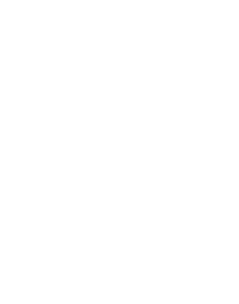
\includegraphics[width=45pt]{redundancy}
\hspace{1.5cm}
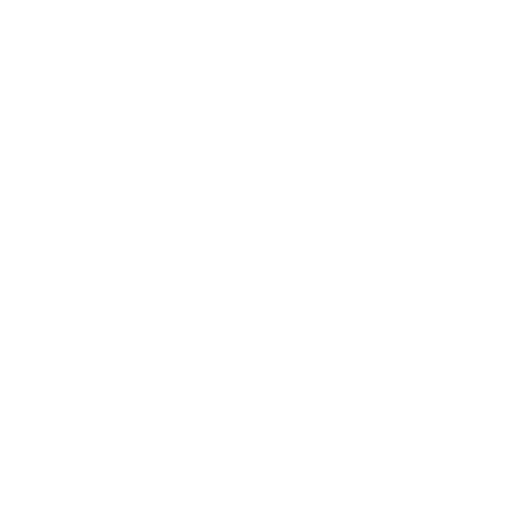
\includegraphics[width=45pt]{tolerance}
\hspace{1.5cm}
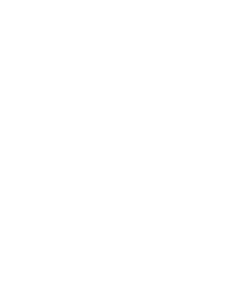
\includegraphics[width=45pt]{load-balance}
\\
\vspace{0.12cm}
\hspace{8pt}\emph{Redundancy}\hspace{38pt}\emph{Fault-Tolerance}\hspace{30pt}\emph{Load Balancing}
\end{center}

\noindent A video streaming service would be able to take advantage of the network and the available speeds and fault-tolerance. As the videos stored on the network would be sharded and spread out on the network, users using the service would always load content from the fastest gridnode swarm with the lowest latency. The implementation needed from the actual video service would be simpler and could rely on the built in redundancy and fault-tolerance of the network, meaning the time and resources needed to implement such as service would also be far lower when compared to a more traditional solution.

\subsection{Compute Cycles}
As the network grows and more gridnodes come online, the compute power available on the network will continuously increase. The scoring algorithms on the network will encourage operators to run gridnodes with a lot of resources - resulting in a network with a constantly increasing storage capacity and available computational power. Using Unigrid tokens, organizations and users will be able to rent these resources and use them for custom workloads and data.

\vspace{0.12cm}
One use case appropriate for this would be a scientific study that needs to run some very complex computationally intensive tasks. In return, the gridnodes offering the service would be awarded a certain amount of Unigrid, as decided by the network. 

Another way to take advantage of the computational power on the network would be to run a container or VPS (Virtual Private Server) on top of the shard groups. Thanks to the redundancy and parity blocks - the network allows for the deployment of containers and server instances that never go offline unintentionally.

\begin{mdframed}[style=textimage]
	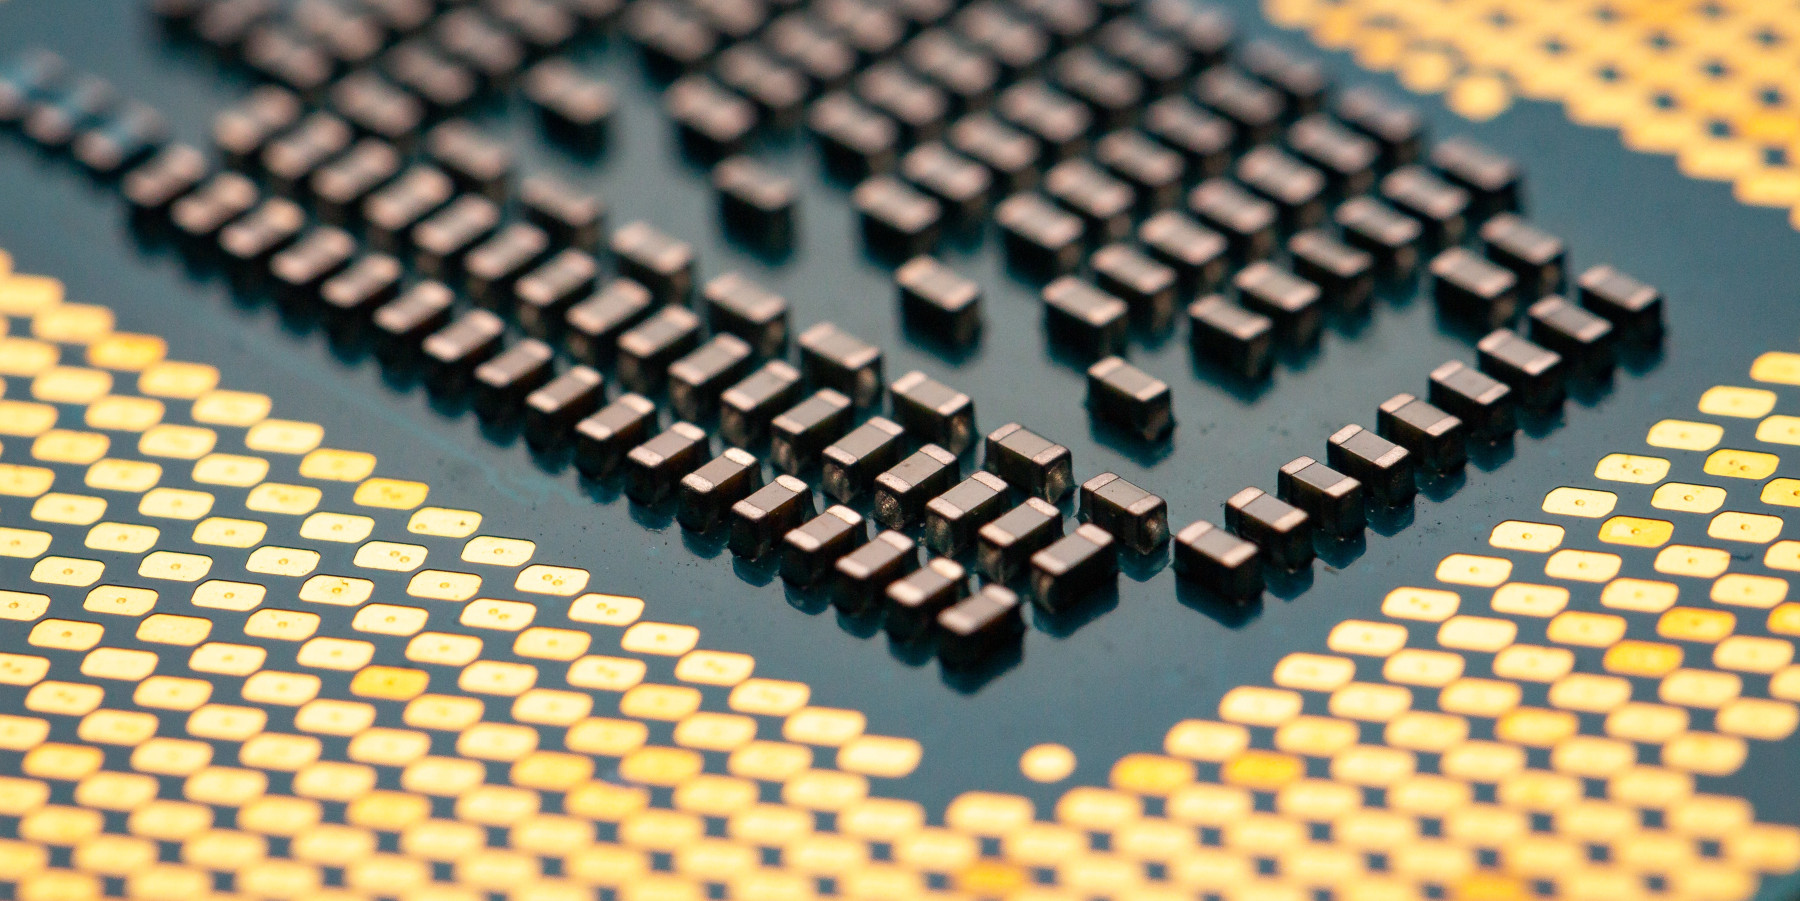
\includegraphics[width=381pt]{compute}
\end{mdframed}

\noindent In future milestones, the Unigrid network will also support GPU workloads. This means that cycles specifically written for graphical processors will also be handled by the gridnodes on the network. As an even more distant goal and when the available technology allows for a working implementation, the foundation also plans to add support for quantum cycles - which would allow the network to process work specifically designed for quantum processors.

\subsection{Domain Registry}
Since Unigrid is its own network, users will also be able to secure and register domain names on the network. The registration fees for a domain will, in turn, be allocated to gridnodes that handle these registrations and the storage of this data. Domain names can even be tethered to a specific Unigrid address - allowing for easy payments to human-readable names, rather than having to enter random Unigrid addresses (which are not nearly as readable).

This opens up a market segment on the Unigrid network for external providers, or entities controlled by The Unigrid Foundation, to develop domain market systems and websites. Systems like these would allow users to buy and trade Unigrid domain names. The network will also provide reverse proxies for ordinary Internet users to be able to access websites and services hosted on the Unigrid network. Rather than accessing \emph{www.someunigridsite.com}, an ordinary Internet user will be able to access the network via the address \emph{proxy.unigrid.org/- www.someunigridsite.com}.

According to John Levine at CircleID \cite{john2018} the domain registrar business is valued at \$3 to \$5 billion per year and growing.

To ease adoption and simplify the process of registering domain names, a simple domain registration interface is planned to be built into the Unigrid wallet and daemon. This will allow users to easily register names directly from the wallet while third party services are developed.

\subsection{Migration}
Connecting directly to the ordinary Internet exposes your personal information to external parties. In order to avoid this leaking of personal data, many Internet users use a VPN (Virtual Private Network). This helps to protect your personal data by creating an encrypted tunnel to the Internet. However, the question is - can you fully trust the VPS provider?

\vspace{0.05cm}
\begin{mdframed}[style=textimage]
	
\includegraphics[width=381pt]{migration}
\end{mdframed}

\noindent When accessing the ordinary Internet via the Unigrid network, a connection is made via a locally running proxy server, assigning a fingerprint to a specific communication channel. A gridnode will pick up this fingerprint and act as the “outlet” for that connection. The data being sent is encrypted. The gridnodes themselves act as a swarm of proxies - meaning nobody actually knows who picks up the data or who is the originating party. This is very different from TOR (onion routing), which sends data via a chain of hops.

The anonymous communication layer is one of the first milestones planned to be developed. This promotes the network recognition and offers a very important use case for new users.

\subsection{Governance}
Control of the network itself and deciding what is allowed and not is handled by the gridnodes and the nodes running on the network. A voting system similar to the governance system in other cryptocurrency projects will be used to vote on important decisions and spork changes. As soon as the foundation changes certain settings on the network, the gridnodes on the network have a choice to either acceppt or reject the change. These settings allow the network to control it's own behaviour. The foundation can add blocks that should be blacklisted on the network and change a lot of different settings that changes the way the different implementations and algorithms used on the network actually behave.

\vspace{0.05cm}
Any major updates to the network itself will also be voted on by the gridnodes. This creates a fully decentralized and democratic network that is controlled 
by it's users - not by a central governing body.

\begin{mdframed}[style=textimage]
	
\includegraphics[width=381pt]{abstract-particles}
\end{mdframed}

\subsection{Past Decentralization Attempts}
Many projects claim decentralization, but in reality most require specialized hardware and do not allow nodes to democratically contribute to the network - some even require written applications and employ a vetting process.

\noindent This effectively moves the centralization to another point of failure rather than solving the underlying problem.

With Unigrid, anyone will be able to join the network and become a gridnode host. This in turn democratizes the network - giving each gridnode a vote on proposals and changes.

\subsection{Market Adoption}
To ensure the financial stability of the the Unigrid Foundation, some departments within the foundation will focus on developing services around or for the Unigrid network. One part of the foundation will work towards developing and providing combined hardware and software solutions that corporations can buy in order to easily get access and contribute to the network. A second part of the foundation will form a legal division. This division will work with the daily legal issues within the foundation but also work towards the goal of supporting start-ups who want to work within the blockchain market. With access to a private data center readily available, the foundation will, as a third service, have the ability to help users contribute to the network by offering data center space for those who can not run gridnodes at home or at their own company. An open VPN service will also be created on the network to gain traction. 

\vspace{0.12cm}
\begin{mdframed}[style=textimage]
	
\includegraphics[width=381pt]{road}
\end{mdframed}

\noindent The Unigrid Foundation will also be working to partner with universities and scientific research organizations. The foundation will allocate a certain percentage of compute cycles and data storage space to these institutions. With many years of teaching experience at a university level available within the foundation, education will be one of the goals with these partnerships. With more knowledge about blockchain at the universities, more students will be able to contribute to the blockchain community as a whole and to the Unigrid network. Since the foundation is based in Gothenburg, close to Chalmers University of Technology, students will also be offered to write their master thesis at the Unigrid Foundation. There are also plans to create grant programs which can be applied to, allowing access to funds from the foundation to further the development and adoption of the network. 

The foundation plan to organize hackathons and similar events to promote growth and development on the Unigrid network. The community will be one of the foundations biggest assets, somewhere where the foundation can look for new hires among the many eager developers and blockchain enthusiasts within the community.

\subsection{Competitive Advantage}
The Unigrid network will keep the cost of data storage and data processing to a minimum. With gridnodes constantly competing for work, costs will be drastically lower than alternative services.

Data on the network is automatically backed up and spread across the network for redundancy. If one gridnode goes down, it's data is accessible via other nodes in the shard group. Consequently, the data is always online and accessible. The network itself will never go offline, allowing continuous and uninterrupted access to your data and apps.

\subsection{Foundational Structure}
The foundation will be overseen by the county administrative board of the region, helping to ensure that assets are properly managed and that the foundation charter is adhered to.

\vspace{0.05cm}
\begin{mdframed}[style=textimage]
	
\includegraphics[width=381pt]{foundation}
\end{mdframed}

\noindent Developing a public utility under a Swedish foundation that is socially beneficial grants several tax benefits and allows the foundation to minimize tax expenditures, increasing funding for internal development and research sponsorship into the fields of distributed communication and storage.

Investments into high-yield assets with additional returns from the Unigrid network will allow the foundation to be self-funding after the initial public sales.

\section{Token Metrics \& Sale}
The Unigrid Foundation is conducting a series of sales rounds in order to finance initial development of the network. Three sales rounds in total will conducted with an additional angel funding round to accredited investors and venture capital firms. The tokens for the angel round are taken from the 20 million tokens up for sale in the first sales round. Angel investors get a discount and are able to buy these tokens at \$0.75 rather than the \$1.00-\$1.25 sales price specified in the actual round. Also, in the event that the foundation sells all 20 million tokens in the initial angel round, the sales round scheduled for October 2021 will not include sales of any tokens from the foundation. Instead, the foundation will shift it's focus to the second sales round scheduled for October 2022. The following sales rounds are planned:

\renewcommand{\arraystretch}{1.5}%
\begin{flushleft}
	\hypersetup{colorlinks = true, urlcolor = black, citecolor = black, linkcolor = black}
	\center \small
	\begin{tabular}{{lrrr}}
		\rowcolor{orange}\color{black}\textbf{Round 1}, Target Date: October 2021\hspace{4cm} & \color{black}Option 1 & \color{black}Option 2\\
		Tokens                               &  10 000 000 & 10 000 000 \\
		\rowcolor{headerbgl}Price            &  \$ 1.00    & \$ 1.25 \\
		Lock Period                          &  1 Year     &  6 Months \\
		\rowcolor{headerbgl}Vesting Schedule &  2 Months   & 2 Months
	\end{tabular}
\end{flushleft}

\renewcommand{\arraystretch}{1.5}%
\begin{flushleft}
	\hypersetup{colorlinks = true, urlcolor = black, citecolor = black, linkcolor = black}
	\center \small
	\begin{tabular}{lrrrrr}
		\rowcolor{orange}\color{black}\textbf{Round 2}, Target Date: October 2022\hspace{1.9cm} & \color{black}Option 1 & \color{black}Option 2 & \color{black}Option 3\\
		Tokens                               &  15 000 000 & 10 000 000 & 10 000 000 \\
		\rowcolor{headerbgl}Price            &  \$ 1.50    & \$ 2.50    & \$ 4.00 \\
		Lock Period                          &  1 Year     &  6 Months  & No Lock-Up \\
		\rowcolor{headerbgl}Vesting Schedule &  2 Months   & 2 Months & N/A 
	\end{tabular}
\end{flushleft}

\renewcommand{\arraystretch}{1.5}%
\begin{flushleft}
	\hypersetup{colorlinks = true, urlcolor = black, citecolor = black, linkcolor = black}
	\center \small
	\begin{tabular}{lrrrrr}
		\rowcolor{orange}\color{black}\textbf{Round 3}, Target Date: April 2023\hspace{2.35cm} & \color{black}Option 1 & \color{black}Option 2 & \color{black}Option 3\\
		Tokens                               &  20 000 000 & 10 000 000 & 10 000 000 \\
		\rowcolor{headerbgl}Price            &  \$ 4.00    & \$ 5.00    & \$ 6.00 \\
		Lock Period                          &  1 Year     &  6 Months  & No Lock-Up \\
		\rowcolor{headerbgl}Vesting Schedule &  2 Months   & 2 Months & N/A 
	\end{tabular}
\end{flushleft}

\vspace{0.6cm}
\noindent Any tokens not sold in each round will be placed under the care of the foundation for future use. Because of the proof of stake nature of the  network, investments for a single entity are capped at three million tokens per investor per round, with a single entity allowed to hold at most 10\% of the total supply.

\noindent Tokens will start being unlocked and accessible when the first official exchange listing of Unigrid occurs. The unlocked amounts and frequencey will follow the specified schedule.

The biggest investors of The Unigrid Foundation will, at the discretion of the foundation, be offered a board seat on the foundation board. This gives bigger investors insight into the dealings of the foundation and allows them to be part of the decision-making process at the board.

\section{Milestones}
The Unigrid Foundation has defined a number of milestones that should be followed when developing the future network. The foundation plans to continuously develop and deploy the network. Having an active community with a live network running allows for the developers to identify potential problems on the network and continuously tests the efficiency and scalability of the implemented solutions.

\begin{itemize}
  \item New "simple" wallet based on Java
  \item Auto updates
  \item Relayed anonymous Internet access
  \item New governance system
  \item Data storage
  \item Compute work (CPU)
  \item Technology demonstration of "Hello world" running on the network
  \item Compute work (GPU)
  \item Technology demonstration of an FTP server running on the network
  \item Domain name service
  \item Technology demonstration of SETI@Home running on the network
\end{itemize}

\noindent Rather than being a list of tasks, the above milestones is a list of goals that the foundation wants to achieve. While the list may still change, the foundation plans to target these goals in the above specified order.

\section{Conclusion}
Since the advent of the Internet in the 1960's \cite{int1997} the Internet can be defined as a collection of nodes (computers) communicating with each other. What The Unigrid Foundation plans is decentralizing these nodes to where anyone can partake in being a host node on the Internet. From the first contact with the network, your data is encrypted and sharded, making it impossible for anyone else to access this data without a key. Browsing across the network is also anonymous - securing your privacy rights.

\vspace{0.1cm}
\renewcommand{\arraystretch}{1.5}%
\begin{flushleft}
	\hypersetup{colorlinks = true, urlcolor = black, citecolor = black, linkcolor = black}
	\center \small
	\begin{tabular}{lrrrrr}
		\rowcolor{orange}\multicolumn{6}{c}{\color{black} \textbf{Worldwide Cloud Service Revenue Forecast \cite{gartner2019} (Billions of U.S. Dollars)}} \\
		\rowcolor{orange} & \color{black}2018 & \color{black}2019   & \color{black}2020 & \color{black}2021 & \color{black}2022 \\
		Business Process Services (BPaaS) \hspace{2.3cm}              &  45.8 &  49.3 &  53.1 &  57.0 &  61.1 \\
		\rowcolor{headerbgl} Application Infrastructure Services (PaaS) &  15.6 &  19.0 &  23.0 &  27.5 &  31.8 \\
		Application Services (SaaS)                                 &  80.0 &  94.8 & 110.5 & 126.7 & 143.7 \\
		\rowcolor{headerbgl} Management and Security Services       &  10.5 &  12.2 &  14.1 &  16.0 &  17.9 \\
		System Infrastructure Services (IaaS)                       &  30.5 &  38.9 &  49.1 &  61.9 &  76.6 \\
		\rowcolor{headerbgl} Total Market                           & 182.4 & 214.3 & 249.8 & 289.1 & 331.2
	\end{tabular}
\end{flushleft}

\vspace{0.6cm}
\noindent Gridnodes are the backbone to the network and an integral role in how the system functions. For the services provided, they will be rewarded. According to the research company Gartner, the total market share for IaaS cloud infrastructure in 2019 was \$38.9 billion with a projected growth to \$76.6 billion by 2022 \cite{gartner2019}. The potential market share for the Unigrid network is enormous as it can potentially offer benefits, functionality and services currently not available with any other alternative.

\section{Closing Thoughts}
This paper covers some of the features of the Unigrid network and why the foundation thinks they are essential for a future Internet that is healthy, stable and scalable. Many of the topics covered only skim the surface of and do not explain many of the intricate details of the underlying implementations. For additional information and for further details on how the network functions on a theoretical level, the base technical Unigrid white paper \cite{wp2021} broadly describes how the foundation plans to implement much of the functionality discussed in this orange paper.

\newpage
\begin{thebibliography}{999}
\bibitem{wp2021}
    Adam Waldenberg, The Unigrid Foundation,
    \emph{"Unigrid: A foundation for a decentralized, consensus-driven, segmented, blockchain-based Internet"},
    \href{https://www.unigrid.org/about}{www.unigrid.org},
    2021.

\bibitem{int1997}
    Barry M. Leiner, Vinton G. Cerf, David D. Clark, Robert E. Kahn, Leonard Kleinrock, Daniel C. Lynch, Jon Postel, Larry G. Roberts, Stephen Wolff,
    \emph{"Origins of the Internet"},
    \href{https://www.internetsociety.org/internet/history-internet/brief-history-internet}{www.internetsociety.org},
    1997.

\bibitem{fort2021}
    Fortune Business Insights,
    \emph{"Cloud Storage Market Size"},
    \href{https://www.fortunebusinessinsights.com/cloud-storage-market-102773}{www.fortunebusinessinsights.com},
    2021.

\bibitem{gartner2019}
    Gartner, Gartner,
    \emph{"Gartner Forecasts Worldwide Public Cloud Revenue to Grow 17.5 Percent in 2019"},
    \href{https://www.gartner.com/en/newsroom/press-releases/2019-04-02-gartner-forecasts-worldwide-public-cloud-revenue-to-g}{www.gartner.com},
    2019.

\bibitem{john2018}
    John Levine, CircleID,
    \emph{"How Big Is The Domain Business"},
    \href{https://www.circleid.com/posts/20180813_how_big_is_the_domain_business/}{www.circleid.com},
    2018.

\bibitem{jeb2019}
    Jeb Su, Forbes,
    \emph{"Amazon Owns Nearly Half Of The Public-Cloud Infrastructure Market Worth Over \$32 Billion: Report"},
    \href{https://www.forbes.com/sites/jeanbaptiste/2019/08/02/amazon-owns-nearly-half-of-the-public-cloud-infrastructure-market-worth-over-32-billion-report/ }{www.forbes.com},
    2019.

\bibitem{young2021}
    Joseph Young, Forbes,
    \emph{"NFT Market Rages On: NFTs Market Cap Grow 1,785\% In 2021 As Demand Explodes"},
    \href{https://www.forbes.com/sites/youngjoseph/2021/03/29/nft-market-rages-on-nfts-market-cap-grow-1785-in-2021-as-demand-explodes/
}{www.gartner.com},
    2021.

\bibitem{mark2019}
    Mark Drake ,Digital Ocean,
    \emph{"Understanding Database Sharding"},
    \href{https://www.digitalocean.com/community/tutorials/understanding-database-sharding}{www.digitalocean.com},
    2019.

\bibitem{jain2021}
    Shruti Jain ,Deloitte,
    \emph{"Can blockchain accelerate Internet of Things (IoT) adoption?"},
    \href{https://www2.deloitte.com/ch/en/pages/innovation/articles/blockchain-accelerate-iot-adoption.html}{www.deloitte.com},
    2021.

\bibitem{wiki2021}
    Wikipedia,
    \emph{"Internet censorship in China"},
    \href{https://www.wikipedia.org/wiki/Internet_censorship_in_China}{www.wikipedia.org},
    2021.
\end{thebibliography}
\end{document}
